% !TEX encoding = UTF-8 Unicode
%Präambel

%Report für große Doukumente. Dieser ist in Kapitel (\chapter{}) aufgeteilt
%\documentclass[12pt, a4paper, ngerman]{report} 

%Article für normale Doumente
\documentclass[12pt, a4paper, ngerman]{article}

%Deutsche Beschreibungen von generiertem Text (table of contents => Inhaltsverzeichnis)
\usepackage[ngerman]{babel}

%Umlaute
\usepackage[utf8]{inputenc}

%Schriftart Helvetica 
\usepackage[scaled]{helvet}

%Seitenränder
\usepackage{geometry}
%top = Abstand nach oben
%left = Abstand nach links
%right = Abstand nach rechts
%bottom= Abstand nach unten
%heapsep= Abstand zwische Kopfzeile und Text
%footskip= Abstand zwischen Text und Fußzeile
\geometry{a4paper, top=25mm, left=30mm, right=25mm, bottom=30mm, headsep=10mm, footskip=12mm}

%Farben nutzen
\usepackage{xcolor}

%Grafiken einbinden
\usepackage{graphicx}

%Zusätzliche Positionsbefehle
\usepackage{float} 

%Die Einrücktiefe bei einem neuen Absatz
\setlength{\parindent}{0pt}


%Fülltext
\usepackage{blindtext}

%Fuer Zitate	
\PassOptionsToPackage{backend=bibtex}{biblatex}
\usepackage[natbib=true,style=numeric]{biblatex}
\usepackage[babel,german=guillemets]{csquotes}
\bibliography{quellen.bib} 

% Aufnahme von \paragraph in das Inhaltsverzeichnis 
\setcounter{tocdepth}{3}  

%Nummerierung vertiefen, \paragraph kommt mit ins Inhaltsverzeichnis
\setcounter{secnumdepth}{4} 

%Feste Tabellen
\usepackage{tabulary}

%caption für nummerierte Tabellenüberschriften
%booktabs für die Steuerung von Linien
\usepackage{caption, booktabs}


%Eigene Kommandos
% Osi Modell
\newcommand{\osi}{ISO/OSI Referenzmodell\xspace}
\newcommand{\fcs}{FCS, Frame Checking Sequence,\xspace}

%Ende Präambel
	
\begin{document}

\begin{titlepage}
		\begin{center}
			
\includegraphics[width=.8\linewidth]{Grafiken/logo_htw.jpg}\\[1cm]    
			\textsc{\LARGE Hochschule für Technik und Wirtschaft \newline Fakultät für Ingenieurwissenschaften}\\[1.5cm]
			\newcommand{\HRule}{\rule{\linewidth}{0.5mm}} \HRule \\[0.4cm] { \huge \bfseries Ausarbeitung Protokolle}\\[0.4cm]
			\HRule \\[1.5cm]

			\begin{minipage}{0.4\textwidth}
				\begin{flushleft} \large
					\emph{Autoren:}\\
					Deniz Kadiogullatri 3553892\\
					Christoph Drost 3576450
				\end{flushleft}
			\end{minipage}
			\hfill
			\begin{minipage}{0.4\textwidth}
				\begin{flushright} \large
					\emph{Betreuer:} \\
					Jonas Vogt, M.Sc.
				\end{flushright}
			\end{minipage}
			\vfill
			{\large \today}
		\end{center}
	\end{titlepage}


%Inhaltsverzeichnis auf eigener Seite
\tableofcontents
\newpage 

\section{Einleitung}
Im Folgenden sollen verschiedene Layer 2 Protokolle für kabelgebundene Netze miteinander verglichen werden. Um die Zusammenhänge besser erklären zu können, möchten wir erst auf das \osi eingehen.
\subsection{Das \osi}
\begin{figure}[h]
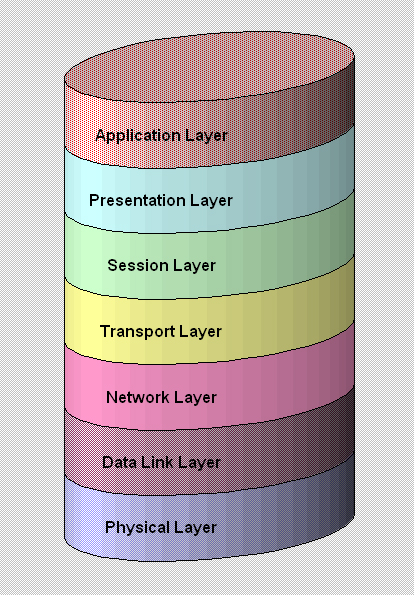
\includegraphics[width=0.5\textwidth]{Grafiken/osi_modell.jpg}
\caption{Das \osi im Überblick \cite{osi_modell}}
\label{osi_modell}
\end{figure} 
Diese Grafik stellt die Schichten des \osi da. Das \osi, (Open Systems Interconnection Model) ist ein allgemeines Kommunikationsmodell,  das die Kommunikation unterschiedlichster Geräte ermöglicht. Es beschreibt ein komplettes Telekommunikationsnetzwerk. Die einzelnen Funktionen sind in 7 Schichten aufgeteilt. 

Das \osi standardisiert die Netzwerk Architektur. Dadurch können Hersteller Lösungen anbieten, die auf der ganzen Welt genutzt werden können. Eine proprietäre Lösung hätte zu Insellösungen geführt. Ein weiterer Vorteil ist, dass die einzelnen Schichten, oder Layer, über Schnittstellen miteinander kommunizieren. Das ermöglicht ein Austauschen einzelner Komponenten, ohne die gesamte Architektur ändern zu müssen.

Da das \osi nur ein Referenzmodell darstellt, müssen die einzelnen Schichten konkret implementiert werden. Diese Implementierungen sind eigene Protokolle. 

\subsection{Der Layer 2}
Der Layer 2, Data Link Layer, setzt auf dem Physical Layer auf und stellt dem Network Layer seine Dienste zur Verfügung. Der Physical Layer beschriebt das Medium über das die Signale übertragen werden. Hier findet noch keine Logik statt. 

Die Aufgaben des Layer 2 im Überblick:
\begin{itemize}
	\item Aufteilung in Pakete
	\item Fehlerkontrolle
\end{itemize} 

\subsubsection{Aufteilung in Frames}
Die Datenblöcke werden im Layer 2 in Frames aufgeteilt. Die Vorteile des Framing sind die schnellere Nutzung eines shared Mediums und dass fehlerhafte Daten nicht komplett übertragen werden müssen.
\subsubsection{Fehlerkontrolle}
Der Data Link Layer führt eine Fehlerkontrolle durch. Dazu zählen eine Suche nach Duplikaten, nach inkorrekt oder unvollständig gesendeten Paketen. Wenn ein Fehler entdeckt wird, wird eine neue Übertragung der Frames angefordert \cite[S. 91]{SWB-107223570}. Die Fehlerkontrolle wird über den \glqq Cyclic Redundancy Check\grqq ~CRC durchgeführt. Dieses Verfahren ist eine Möglichkeit zur Prüfsummenberechnung, die beim Sender und der Senke durchgeführt wird. Sind beide Prüfsummen gleich, kann angenommen werden, dass das Frame korrekt übertragen wurde. 

Die Frames werden mit Sequence Numbers durchnummeriert. Der Empfänger prüft, ob die Frames in der richtigen Reihenfolge ankommen. Bei einer \glqq out-of-sequence transmission\grqq ~kann von einem verlorenen Frame ausgegangen werden, das entsprechende Frame wird neu angefordert, bzw. Layer 3 wird benachrichtigt.
\section{Die Layer 2 Protokolle im Überblick}

\subsection{Ethernet}
Ethernet ist ein weit verbreitetes Layer 2 Protokoll. 90\% aller lokal installierten Netzwerke sind mit Ethernet realisiert\cite{SWB-097965316}. Ethernet wurde ursprünglich für die Anbindung eines Druckers bei der Firma Xerox Corporation entwickelt. Die damalige Übertragungsgeschwindigkeit von 2,94 Mbit/s wurde auf aktuell 100 Gbit/s gesteigert, weitere Steigerungen sind zu erwarten.

Die Daten werden im Ethernet über einen eigenen Übertragungskanal transportiert. Kollisionen werden durch \glqq CSMA/CD\grqq ~entdeckt, bzw. aufgelöst. Die Übertragung läuft gleichberechtigt und verbindungslos. Die Daten werden an alle Teilnehmer weitergeleitet, diese vergleichen die Empfängeradresse mit ihrer eigenen und verwerfen die Frames, die nicht an sie adressiert sind. Diese Aussage kann eingeschränkt werden, da Switche die Daten nur an Ports leiten, an denen die entsprechenden Senken angeschlossen sind. 

\subsubsection{Gebräuchliche Übertragungsmedien des Ethernet}
\begin{figure}[H]
\begin{minipage}[hbt]{.28\linewidth}
	\centering
	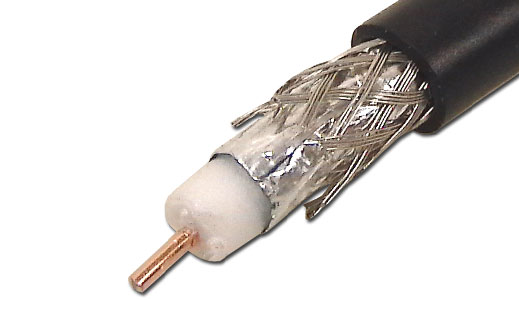
\includegraphics[width=0.9\linewidth]{Grafiken/koaxkabel.png}
	\caption{Koaxkabel \cite{koax_kabel}}
	\label{koaxkabel}
\end{minipage}
\hfill
\begin{minipage}[hbt]{.28\linewidth}
	\centering
	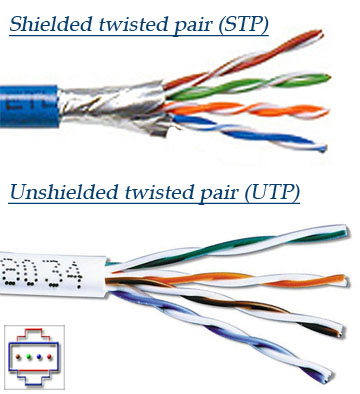
\includegraphics[width=0.9\linewidth]{Grafiken/twistetPair.jpg}
	\caption{Twistet Pair Kabel \cite{tw_kabel}}
	\label{twkabel}
\end{minipage}
\hfill
\begin{minipage}[hbt]{.28\linewidth}
	\centering
	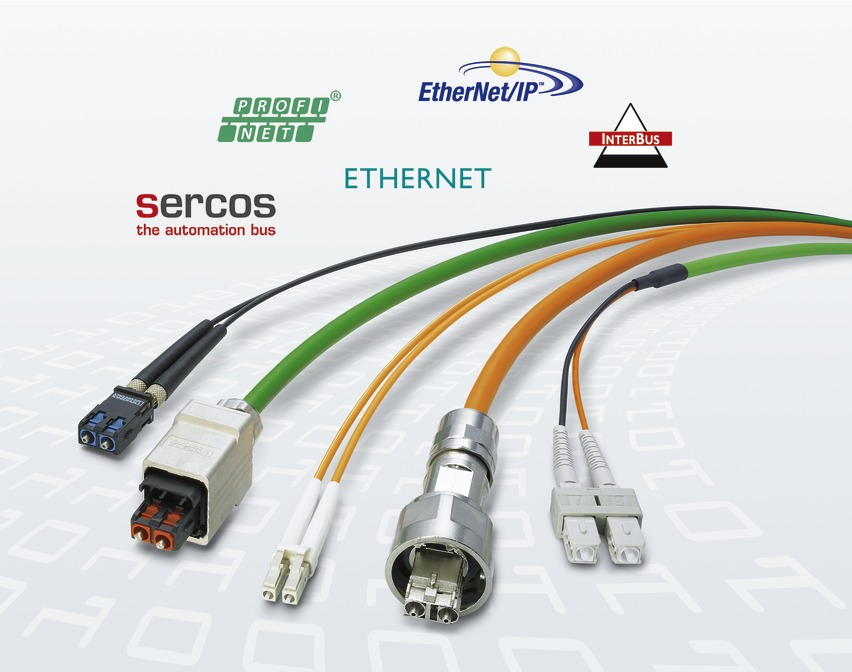
\includegraphics[width=0.9\linewidth]{Grafiken/lwl_leiter.jpg}
	\caption{Lichtwellenleiter \cite{lwl_leiter}}
	\label{lwlleiter}
\end{minipage}
\end{figure}
 
Historisch gesehen muss das Koaxialkabel als Medium des Ethernet genannt werden. Das Koaxkabel wurde 1990 mit der Einführung von 10BaseT (IEEE 802.3i) durch Unshielded Twisted Pair Kabel ersetzt. Ab 1998 wurden mit der Einführung des Gigabit Ethernet auch Lichtwellenleiter genutzt. 

\subsubsection{Adressierung \label{ethernet_adresse}}
 Ethernet nutzt zur Adressierung von Teilnehmern deren MAC-Adresse. MAC-Adressen, Media Access Control Adress, sind Hardwareadressen und werden weltweit eindeutig vergeben. Sie bestehen aus 6 Byte und sind nach folgendem Muster aufgebaut: 
 
 Hersteller--Hersteller--Hersteller--xx--xx--xx 

Der Herstellerteil, auch Organizationally  Unique Identifier (OUI), wird von der IEEE vergeben. Jeder Hersteller hat seinen eigenen Bereich, der durch die ersten 3 Bytes bestimmt wird. Die letzten 3 Bytes werden vom Hersteller selber vergeben. Dabei ist der Hersteller für die eindeutige Vergabe der letzten 3 Bytes verantwortlich. Einige Hersteller haben mittlerweile mehrere eigene Bereiche.

\subsubsection{Zugriff auf das Medium}
Historisch gesehen nutzt Ethernet das Übertragungsmedium als Shared Medium. Die einzelnen Teilnehmer wurden am selben Koaxialkabel über T-Stücke angeschlossen. Um Kollisionen zu vermeiden, wurde ein geeignetes Verfahren zur Vermeidung benötigt. Von einer Kollision spricht man, wenn mehrere Teilnehmer gleichzeitig auf das Medium zugreifen würden, also Signale aussenden. Die Signale würden sich gegenseitig überlagern und wären nicht mehr nutzbar. Bei Ethernet wird CSMA/CD eingesetzt. Bei diesem Verfahren wird vor dem Senden geprüft, ob die Leitung frei ist. Erst wenn die Leitung frei ist wird gesendet (Carrier Sense). Wenn zufällig mehrere Teilnehmer gleichzeitig ein Signal aussenden (Multiple Access) kommt es dennoch zu Kollisionen. Der/Die Sender prüfen während dem Senden, ob es zu Kollisionen kommt (Collision Detect) und brechen ihre Übertragung im Fall einer Kollision ab. Nach einem Abbruch wird eine zufällige Zeit gewartet bis erneut gesendet wird. Der Grund, warum es trotz diesem Verfahren zu Kollisionen kommen kann, ist die Signallaufzeit. Die Signale brauchen eine gewisse Zeit um über die Leitungen übertragen zu werden. 

In seinen Anfangszeiten übertrug Ethernet im Halbduplex Verfahren. Das bedeutet, dass ein Übertragungskanal zum Senden und zum Empfangen genutzt wird. Dadurch halbiert sich natürlich im schlimmsten Fall die Datenrate. Mit der Einführung von Twisted Pair Kabeln und Lichwellenleitern wurde Ethernet auf den Vollduplex Betrieb umgestellt. Dadurch konnte die Übertragungsrate gesteigert werden und Kollisionen wurden unwahrscheinlicher.
\begin{figure}[H]
	\centering
	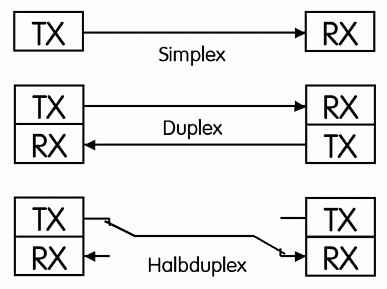
\includegraphics[width=0.4\linewidth]{Grafiken/duplex.jpg}
	\caption{Unterschied der Duplex Übertragungen \cite{duplex}}
	\label{duplex}
\end{figure}
 
 \subsubsection{Frames}
Um Daten über Ethernet übertragen zu können werden sie in Frames aufgeteilt. Der Vorteil daran ist, dass ein Sender bei großen Übertragungen nicht das gesamte Netzwerk belegt und dass bei einer fehlerhaften Übertragung nur einzelne Frames neu versandt werden müssen. Der Ausdruck Frame kann wörtlich genommen werden. Die Nutzdaten werden in einen Rahmen (Frame) eingepackt.

Ein Frame ist folgendermaßen aufgebaut:
\begin{itemize}
	\item Die Präambel 
	\item Die Hardware Quell- und Zieladresse
	\item Ein Typ- oder Längenfeld
	\item Nutzdaten
	\item Eine Checksumme
\end{itemize}
\begin{figure}[H]
	\centering
	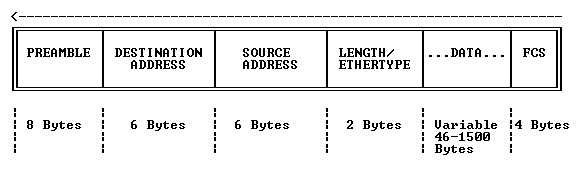
\includegraphics[width=0.9\linewidth]{Grafiken/ethernet_frame.jpg}
	\caption{Ethernet 802.3 Frame \cite{ethernet_frame}}
	\label{ethernet_frame}
\end{figure}

\paragraph{Präambel}
Die Präambel enthält eine Bitfolge, die dem Empfänger signalisiert, dass ein Rahmen ankommt. Die Präambel besteht aus 8 Bytes mit einer alternierenden Folge aus 0 und 1. Die letzten 2 Bits im letzten Byte sind immer 1. Hier besteht ein kleiner Unterschied zwischen DIX und IEEE. Obwohl die Bitfolgen die gleichen sind, ist die Präambel im IEEE Standard formell in die 7 Byte lange Präambel und den 1 Byte langen Start-of-Frame-Delimiter aufgeteilt.
Sie dient u.a. zur Synchronisation der Empfängerstationen. 

\paragraph{ Die Hardware Quell- und Zieladresse}
Die Adressen sind MAC Adressen. Ihr Aufbau ist bereits in \ref{ethernet_adresse} beschrieben worden. Ein Ethernet Frame hat sowohl die Ziel- als auch die Senderadresse.

\paragraph{Typ- oder Längenfeld}
Um zu verstehen, warum beide Bezeichnungen möglich sind muss man wieder die Historie betrachten. Die DIC Gruppe nutzte das Feld als Typfeld. Dort wurde definiert, welche Daten des höheren Layers übertragen werden.  Im Standard IEEE 802.3 wird das Feld als Längenfeld genutzt. Um welches Feld es sich dabei genau handelt, kann anhand der Größe festgestellt werden. Die Typenbezeichnungen beginnen ab 1635 (0x0600). Ein Wert darunter kann nur eine Längenangabe sein. Jumbo- und Super Jumboframes sind abseits von IEEE 802.3 definiert.

\paragraph{Nutzdaten}
Die Nutzdaten sind die Daten, die eigentlich übertragen werden sollen. Das Feld mit den Nutzdaten hat eine Mindestlänge von 46 Byte  und eine Maximallänge von 1500 Byte. Die Mindestlänge kommt von der Anforderung des CSMA/CD, wonach ein Frame mindestens 64 Byte haben muss. Zieht man von den 64 Byte die Headerlänge (14 Byte) und die Checksumme (4 Byte) ab kommt man auf 46 Byte. Wird die Mindestlänge der Nutzdaten unterschritten, wird das Feld mit sogenannten Pads aufgefüllt. Sie haben den Wert 00.
\paragraph{Checksumme \label{checksumme}}
Die letzten 4 Bytes eines Ethernet Frames sind das \fcs oder Frame Checking Field. Das FCS dient der Sicherstellung, dass der Frame korrekt übertragen wurde. Der Inhalt dieses Feldes wird mit durch CRC-Algorithmus errechnet. Sowohl Sender als auch Empfänger wenden ihn an, kommen bei der Berechnung unterschiedliche Werte heraus, kann davon ausgegangen werden, dass auf Layer 1 Bits verfälscht wurden. Neben dem CRC Verfahren werden zur Prüfung auch andere Kriterien zur Prüfung eines Frames angewandt:
\begin{itemize}
	\item Die Framelänge stimmt nicht mit dem Längenfeld überein (nur bei IEEE 802.3)
	\item Die Framelänge ist kein ganzzahliges Vielfache eines Bytes
\end{itemize}


\subsubsection{Topologie}
Ethernet ist keiner bestimmten Netzwerk Topologie zuzuordnen. Heute gebräuchlich ist eine Sterntopologie, andere Formen sind aber auch möglich.   

\subsection{LAPD}
LAPD, Link Access Procedure on the D-channel ist auch ein Protokoll der Schicht 2. Es wird genutzt um Layer 3 Informationen zwischen den Teilnehmer des ISDN Netzwerks zu übertragen. Für diese Übertragung wird der D-Kanal genutzt.

\subsubsection{Gebräuchliche Medien des LAPD}
Der Layer 1 unter LAPD wird durch den $S_0$ und den $U_{K0}$ Bus beschrieben. Für  $S_0$ werden üblicherweise 4 Draht Kupfer Verkabelungen verwendet, für $U_{K0}$ eine Kupfer Doppelader.
\begin{figure}[H]
\begin{minipage}[hbt]{.35\linewidth}
	\centering
	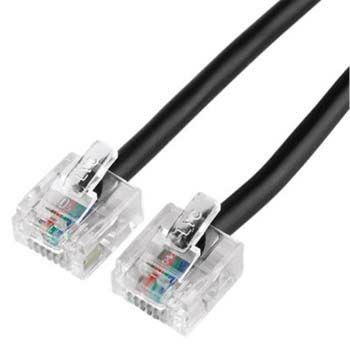
\includegraphics[width=0.9\textwidth]{Grafiken/isdn_kabel.jpg}	
	\caption{Ein typisches IDSN Kabel  ($S_0$) \cite{isdn_kabel}}
	\label{isdn_kabel}\end{minipage}
\hfill
\begin{minipage}[hbt]{.65\linewidth}
	\centering
	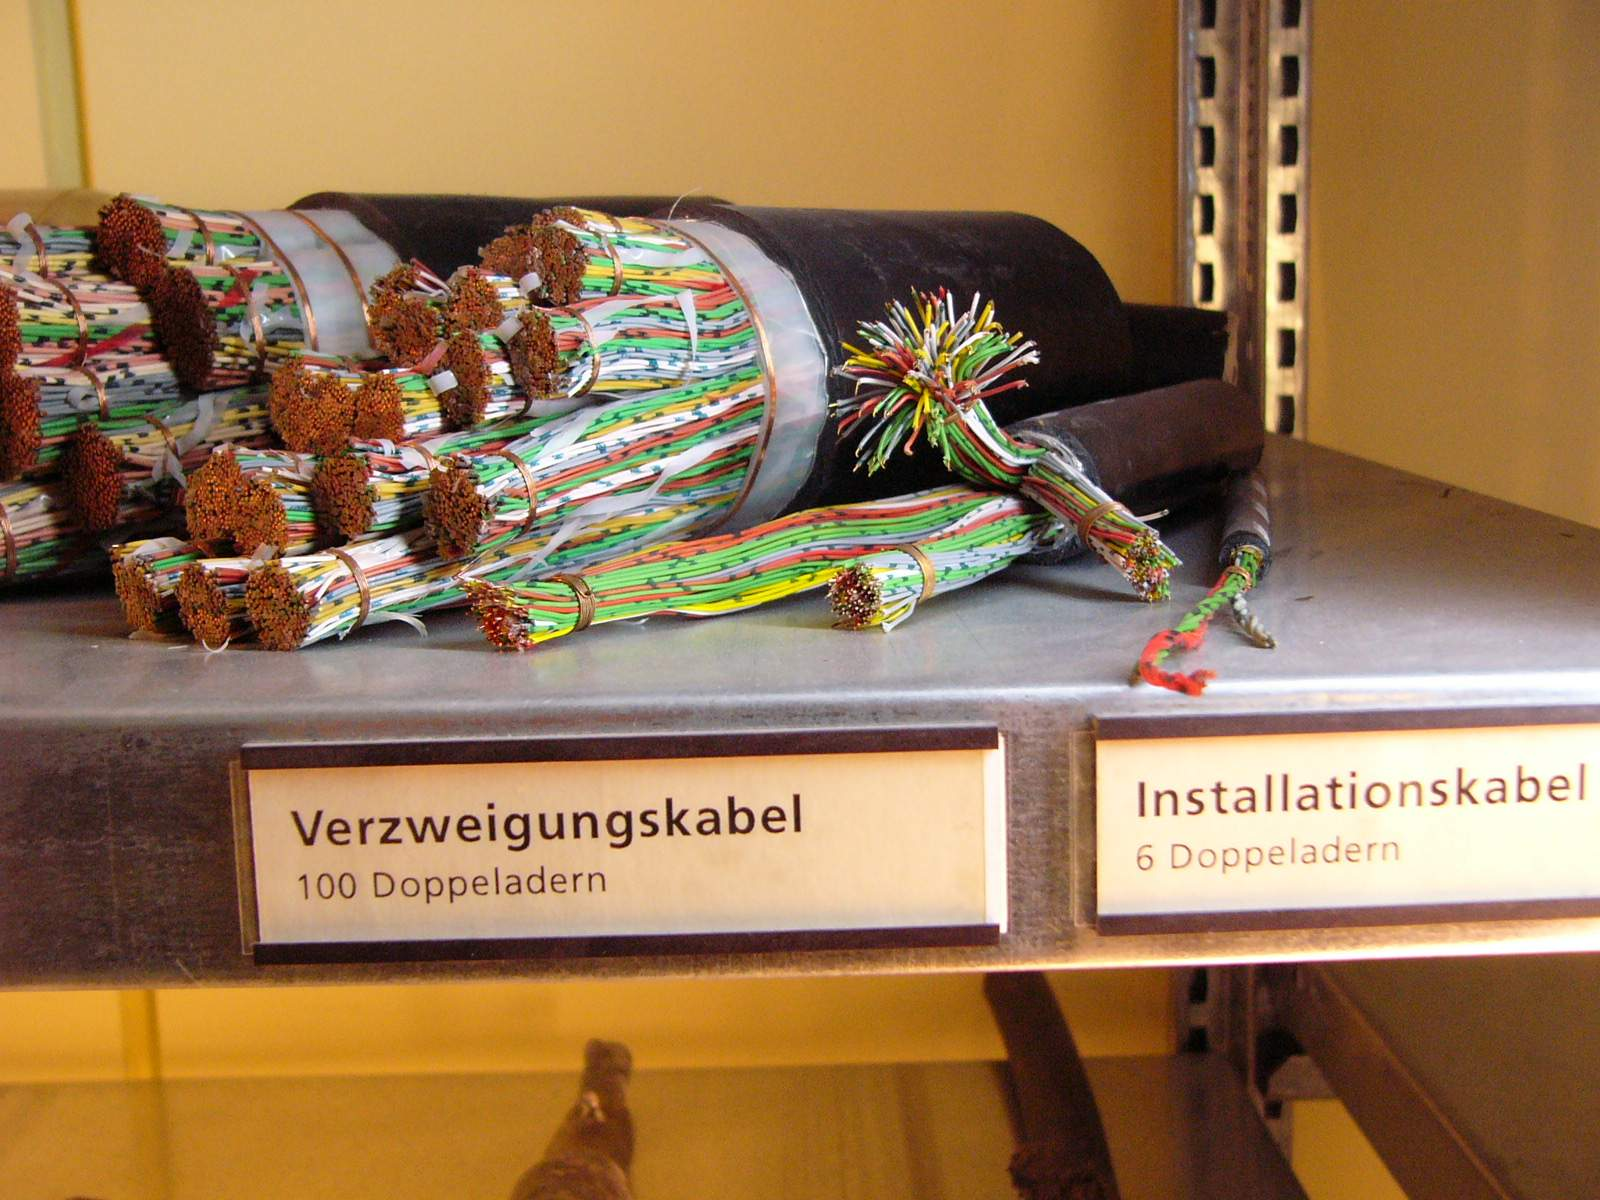
\includegraphics[width=0.9\linewidth]{Grafiken/kuperkabel.jpg}
	\caption{Kupferkabel im Überblick \cite{cu_doppelader}}
	\label{cu_kabel}
\end{minipage}
\end{figure}


\subsubsection{Der D-Kanal}
Der D-Kanal wird im ISDN zur Signalisierung genutzt. Er stellt 16 kbit/s zur Verfügung. Signalisieren bedeutet, dass der Teilnehmer und die Vermittlungsanlage Informationen austauschen. Das können Informationen sein, ob der Teilnehmer verfügbar ist, oder auch Informationen mit denen ein Gespräch aufgebaut wird. Im Gegensatz zu den B-Kanälen, über die Nutzdaten, wie z.B. Sprache, übertragen wird, kommunizieren über den D-Kanal nur Prozessoren.

\subsubsection{Der Zugriff auf das Medium}
LAPD ist das Signalisierungsprotokoll des ISDN. An einem $S_0$ Bus teilen sich bis zu 8 Teilnehmer einen D-Kanal. Der Zugriff durch die Teilnehmer ist priorisiert. Zur Zur Regelung, welcher Teilnehmer bevorrechtigt ist, gilt, je mehr logische Einsen den Teilnehmer identifizieren, desto niedriger ist die Priorität. So kann man sagen, dass der D-Kanal als Shared Medium genutzt wird. Um zu überprüfen, ob eine Kollision stattgefunden hat, gibt es den E-Kanal. Auf diesen wird der D-Kanal durchgeschleift. Der Teilnehmer kann anhand vom E-Kanal überprüfen, ob die Informationen, die er gesendet haben noch einmal bei ihm ankommen. Ist das der Fall, kann er davon ausgehen, dass es zu keiner Kollision mit den Signalen eines anderen Teilnehmers gekommen ist.

Der $S_0$ Bus arbeitet in einem Vollduplexverfahren vgl. Abbildung ~\ref{duplex}. Die Teilnehmer teilen sich das Medium über Zeitschlitze. 

\subsubsection{Adressierung \label{tei}}
LAPD nutzt zur Adressierung der Teilnehmer den TEI, Terminal Endpoint Identifier. Der TEI wird entweder durch eine feste Einstellung im Endgerät oder durch die Vergabe der Vermittlungsstelle vergeben. Er besteht aus 7 Bit. Der TEI ist im normalen Betriebszustand eindeutig, darf aber nicht mit der Rufnummer verwechselt werden.

\subsubsection{Frames}
LAPD teilt die Daten der Schicht 3 in Frames auf. Dabei werden unterschiedliche Frametypen benutzt. Ein Frame ist ist folgendermaßen aufgebaut:

\begin{itemize}
	\item Blockbegrenzung
	\item Adressfeld
	\item Steuerfeld
	\item Daten
	\item Blockprüfung
	\item Blockbegrenzung
\end{itemize}

\begin{figure}[H]
	\centering
	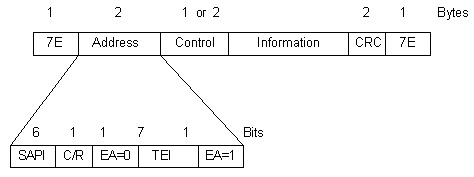
\includegraphics[width=0.9\linewidth]{Grafiken/lapd_frame.jpg}
	\caption{LAPD Frame \cite{lapd_rahmen}}
	\label{lapd_frame}
\end{figure}

\paragraph{Blockbegrenzung \label{blockbegrenzung}}
Die Blockbegrenzung ist eine Byte, das aus eine Bitkombination besteht, die im restlichen Block nicht vorkommt. Sie stellt den Anfang und das Ende des Blocks dar. \textcolor{red}{\textbf{Sollen wir das noch genauer ausführen?}}  S.448 Technik der Netze.  

\paragraph{Adressfeld}
Das Adressfeld besteht aus 2 Bytes. Es enthält den SAPI und den TEI, die je 1 Byte groß sind. Die Größe 1 Byte ist eigentlich ungenau, da man die Bytes wieder genauer aufteilen kann. Jedes dieses Bytes hat ein EA (Extended Adress), damit wird angegeben, ob dem Byte noch weitere folgen. Der SAPI, Service Access Point Identifier,  identifiziert die Dienste der Schicht 2. Er besteht aus 6 Bit, zusätzlich sind in dem Byte das C/R Bit und das EA Bit. Das C/R-Feld kennzeichnet, ob das Paket eine Anweisung (Command) für den Empfänger enthält oder ob es eine Antwort (Response) auf eine zuvor erhaltene Anweisung enthält. 

Aktuell sind 3 Typen des SAPI definiert \cite{SWB-098672061}. 
\begin{itemize}
	\item Die gesicherte Übermittlung von Signalisierungsinformationen (SAPI 0)
	\item Die Übertragung von paketvermittelteten Daten (SAPI 16)
	\item Die Festlegung von eindeutigen TEI (SAPI 63)
\end{itemize}



Der TEI wurde bereits in~\ref{tei} genauer beschrieben. Im Byte des TEI wird EA = 1 gesetzt, da der TEI das letzte Adress Byte ist.

\paragraph{Steuerfeld}
LAPD kennt 4 Rahmentypen. Sie haben verschiedene Funktionen, die im Steuerfeld gekennzeichnet werden. Die Informationen zu dem Steuerfeld stammen komplett aus \cite{SWB-098672061}.

\subparagraph{I-Rahmen}
Der I-Rahmen, Informationsrahmen, dient der Übermittlung von Schicht 3 Informationen. Der I-Rahmen ist der einzige, der einen Sendefolgezähler enthält.

\subparagraph{S-Rahmen}
Der S-Rahmen, Steurrahmen, dient zum Quittieren von empfangenen Rahmen. Mit ihm werden außerdem Zustandsmeldungen (z.B. empfangsbereit) gesendet und bei groben Protokollfehlern andere Rahmen abgewiesen.

\subparagraph{U-Rahmen}
Der U-Rahmen, umnummerierter Rahmen, dient der Übertragung von Steuerkriterien, für die eine Nummerierung nicht möglich oder nicht nötig ist. Beispielsweise kann man dafür das Kommando für die Initialisierung (SABME) einer Schicht 2 Verbindung, oder die Abweisung von fehlerhaften Rahmen (FRMR) nennen.

\subparagraph{UI-Rahmen}
Der UI-Rahmen, umnummerierter Informationsrahmen, ist eine Spezialität des LAPD Protokolls. Er wird für für spezielle Prozeduren im Zusammenhang mit der P-MP-Konfiguration am Basisanschluss benötigt und überträgt die Informationen des Layer 2 (TEI Management) oder des Layer 3 (kommender Ruf). Er wird genutzt wenn vorher noch keine Layer 2 Verbindung eingerichtet wurde. UI-Rahmen werden nicht quittiert.

\paragraph{Daten}
Welche Daten übertragen werden, wird im Steuerfeld geregelt. Die reine Übertragung von Layer 3 Daten erfolgt nur in I-Blöcken. Die Blöcke werden nummeriert und von der Gegenseite bestätigt. Die Bestätigung kann durch einen I-Block oder durch einen S-Block bestätigt werden. Wie oft eine Bestätigung zu erfolgen hat, wird durch die Fenstergröße geregelt. Hier sind Werte zwischen eins und sieben möglich. Das Senden von weiteren Frames ist nur möglich, wenn die vorherigen bestätigt wurden. Bei einem Standard ISDN Basisanschluss ist die Fenstergröße eins, bei einem Primärmultiplexanschluss beträgt die Fenstergröße sieben. Das bedeutet, dass bei einem ISDN Basisanschluss nur ein Frame gesendet werden darf, wenn der vorherige bestätigt wurde. Bei einem Primärmultiplexanschluss können sieben Frames gesendet werden, bevor die erste Bestätigung erfolgt sein muss. Erfolgt die Bestätigung von einem Frame, kann ein weiteres gesendet werden.

Ein I-Block darf maximal 260 Byte groß sein. Daraus ergibt sich eine maximal Gesamtgröße von 268 Byte pro LAPD Frame, wenn I-Blöcke genutzt werden.

\paragraph{Blockprüfung}
Die Blockprüfung findet bei sowohl beim Sender, als auch beim Empfänger statt. Die \fcs wird vom Sender errechnet und in das entsprechende Feld geschrieben. Der Empfänger errechnet sie auch und vergleicht es mit der des Senders. Unterscheiden sich die Werte, kann von einem Fehler bei der Übertragung ausgegangen werden. Die Größe der \fcs ist auf zwei Byte festgelegt.
 
\paragraph{Blockbegrenzung}
Siehe ~\ref{blockbegrenzung}.
 
\subsection{PPP}
Router - Router und Host - Netzwork Verbindungen über synchrone und asynchrone Kreise. Enthält ein Protokoll Feld um das Network Layer Protokoll zu Identifizieren \cite[S. 102]{SWB-107223570}  

Während in einzelnen Gebäuden meist LAN zum Einsatz kommen, werden für die weitreichende Verbindungen meist Punkt-zu-Punkt-Standleitungen eingesetzt. Diese Leitungen verbinden weit entfernte Router miteinander. Hinter diesen können LAN mit mehren Hosts wie Personal-Computer, Workstation oder Server angeschlossen sein. Die Verbindung in die Außenwelt von diesen LAN aus, wird eben genau über diese Router laufen. Und hier kommt das PPP (Point-to-Point Protocol) zum Einsatz.

PPP ist in RFC 1661 definiert und wurde in mehreren anderen RFC, wie in RFC 1662 und 1663, weiter ausgearbeitet.

Das Protokoll unterstützt Fehlererkennung, dynamische IP-Adressen Vergabe bei Verbindungsaufbau, Berechtigungsprüfung und mehrere Protokolle.

Das PPP umfasst des Weiteren noch ein ganzes weiteres Protokoll das zum Aktivieren und Testen einer Leitung als auch zum Verhandeln von verschiedenen Parametern die für das PPP wichtig sind und zum Beenden nicht mehr gebrauchten Verbindungen verwendet wird. Die Aushandlung findet über ein eigenes Protokoll das sogenannte Link Control Protocol, im folgenden kurz als LCP bezeichnet, statt. LCP wird innerhalb des PPP Frames als Nutzdaten übertragen.

Ausserdem ermöglicht PPP es der Vermittlungsschicht (Networklayer) das für auf dieser Schicht laufende Protokoll, von diesem Protokoll unabhängige Optionen auszuhandeln, diese nennt man Network Control Protocol (NCP), so das auf jeder unterstützten Vermittlungsschicht ein anderes NCP laufen kann. 

Beispiele für NCP sind IPCP, AppleTalk Control Protokoll oder IPXCP. Das IPCP steht für IP Control Protocol und wird zur unter anderem zur IP-Vergabe genutzt.


\subsubsection{LCP Verhandlung}


Das Verbindungssteuerungs-Protokoll (Link-Control Protolcol - LCP) des PPP stellt eine Methode für die Etablierung, Konfigurierung, Verwaltung und Beendigung einer Punkt-zu-Punkt-Verbindung zur Verfügung. LCP durchläuft vier einzelne Phasen:
In der ersten Phase erfolgt der Verbindungsaufbau, und die Konfiguration wird ausgehandelt. Bevor irgendwelche Datagramme der Vermittlungsschicht (z.B. IP) ausgetauscht werden können, muß LCP die Verbindung erüffnet und Konfigurationsparameter ausgehandelt haben. Diese Phase ist beendet, wenn sowohl ein Frame gesendet als auch einer empfangen wurde, der die Konfigurationsbestöätigung enthält.
Dann wird die Verbindungsqualität ermittelt. Diese Phase ist optional. In dieser Phase wird die Verbindung getestet, um festzustellen, ob die Qualität dafür ausreicht, daß die Protokolle der Vermittlungsschicht gestartet werden können. LCP kann die Übertragung von Protokoll-Informationen der Vermittlungsschicht so lange hinauszögern. bis diese Phase beendet ist.
Zu diesem Zeitpunkt erfolgt die Konfigurationaushandlung des Vermittlungsschicht-Protokolls. Nachdem LCP die Phase der Qualitätsprüfung beendet hat, können die Vermittlungsschicht-Protokolle vom entsprechenden NCP einzeln konfiguriert werden und jederzeit gestartet oder beendet werden. Wenn LCP die Verbindung beendet, informiert es die Protokolle der Vermittlungsschicht, damit diese entsprechende Schritte einleiten.
Zuletzt erfolgt die Verbindungsbeendigung. LCP kann die Verbindung jederzeit beenden. Eine Verbindung wird im allgemeinen auf Anforderungen eines Benutzers beendet, kann aber auch aufgrund eines physischen Ereignisses beendet werden, z.B. wenn das Trägersignal verloren geht oder ein Timer abläuft.
Es gibt drei Klassen von LCP-Frames. Verbindungsaufbau-Frames dienen dazu, eine Verbindung aufzubauen und zu konfigurieren. Verbindungsbeendigungs-Frames dienen dazu, eine Verbindung zu beenden, während Verbindungsverwaltungs-Frames eine Verbindung verwalten und debuggen.

Diese Frames werden für die Durchführung der einzelnen LCP-Phasen benötigt.

Das LCP befasst sich nicht mit den Optionen selbst die für Schicht-2 ausgehandelt werden sondern nur wie sie ausgehandelt werden. Ein Prozess kann seine Optionen einem anderen vorschlagen und dieser kann dann entscheiden ob er alle annimmt oder nur einige annimmt oder sie ganz abschlägt. Es gibt in RFC 1661 elf verschiedene Typen von LCP-Rahmen die diese verhalten festhalten. 

Im folgenden die einzelnen Typen und ihre Bedeutung:

\begin{itemize}
	\item Configure-request	- Liste der vorgeschlagenen Optionen und Werte
	\item Configure-ack		- Alle Optionen werden angenommen
	\item	Configure-nak		- Einige Optionen werden nicht angenommen
	\item Configure-reject	- Einige Optionen können nicht Verhandelt werden
	\item Terminate-request	- Anforderungen zum Trennen der Verbindung
	\item Terminate-ack		- Verbindung wurde getrennt
	\item Code-reject		- Unbekannte Anforderungen erhalten
	\item Protocol-reject		- Unbekanntes Protocol angefordert
	\item Echo-request		- Anforderungen, den Rahmen zurückzusenden
	\item Echo-reply		- Rückgabe des Rahmens
	\item	Discard-request	- Rahmen verwerfen (für Testzwecke)
\end{itemize} 



\subsubsection{Verbindungsablauf des PPP}

Im folgenden durchlaufen wir die verschiedenen Zustände des Verbindungsaufbaus bis hin zum Abbau der Verbindung anhand der unten gezeigten Zeichnung.
Als ersten ist die Leitung tot. Das bedeutet es existiert kein Träger auf der physikalischen Ebene und auch keine Verbindung auf der Bitübertragungsschicht.
Nachdem eine physikalische Verbindung aufgebaut worden ist wechselt der Zustand zu Aufbauen. Genau in diesem Augenblick beginnt dann die Verhandlung der LCP Optionen. Wenn diese erfolgreich sein sollten können nun die beiden Parteien die mit einander kommunizieren möchten ihre Identität prüfen. Das heisst der Zustand wechselt auf Authentifizieren. Falls dieser Fall nun fehlschlägt wird die Verbindung Beendet, dh. auch der Zustand ändert sich und der Träger wird wieder freigegeben. Somit wären wir wieder im Ausgangszustand. Im Gegengesetzten Fall würde der nächste Zustand Netz heissen und das entsprechende NCP-Protokolle aufgerufen werden um die Vermittlungsschicht zu konfigurieren. Nach dem die Konfiguration erfolgreich abgeschlossen ist wechselt der Zustand nach Öffnen in der die eigentliche Datenübertragung stattfindet. Wenn diese Beendet ist und alle Daten erfolgreich übertragen worden sind kann die Verbindung wie bereits oben geschrieben Beendet werden.

\begin{figure}[H]
	\centering
	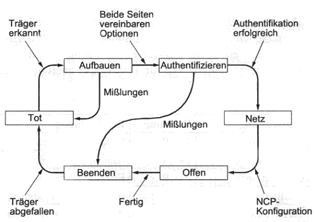
\includegraphics[width=1\textwidth]{Grafiken/ppp.jpg}	
	\caption{Übersicht PPP Verbindungsaufbau \cite{*}}
	\label{aufbau_ppp-verbindung}
\end{figure}


\subsubsection{Frames}

Das PPP besitzt eine Rahmenbildungsmethode die Anfang und Ende eines jeden Rahmens kennzeichnet. Diese übernimmt ebenfalls die Aufgabe der Fehlererkennung

Der Rahmen besteht aus insgesamt sieben Feldern. Dazu gehören Flag, Adress, Steuerung,  Protokoll, Nutzdaten, Prüfsumme und wieder Flag.

\begin{figure}[H]
	\centering
	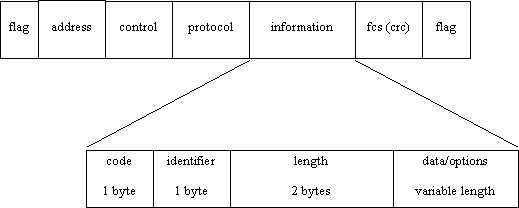
\includegraphics[width=1\textwidth]{Grafiken/ppp-frame.jpg}	
	\caption{Darstellung eines PPP Frames \cite{*}}
	\label{ppp_frame}
\end{figure}

\paragraph{Flag}

Das Flag besteht am Anfang wie am Ende aus einem Byte (011111110) dieses wird mit der Byte-Stuffing-Methode aufgefüllt, um zu verhindern das im Datenfeld eines Frames eine Bitfolge als Sternzeichen interpretiert werden. Das erste Byte ist somit das Startbyte für einen Rahmen. Am Ende eines Rahmens wird die selbe Bitfolge gesendet und zu kennzeichnen das der Frame zu Ende ist.


\paragraph{Adress}

Das Adressfeld steht immer auf einem festen Wert und zwar aus acht mal eins. Dies dient dazu das alle Stationen den Rahmen akzeptieren und zum vermeiden das Verbindungsadressen zugewiesen werden müssen. Da dieses Feld in der Standartkonfiguration immer gleich ist, gibt es wie auch bei dem Steuerungsfeld einen die Möglichkeit zwischen zwei Parteien diese Felder einfach entfallen zu lassen und damit zwei Byte pro Rahmen einzusparen.


\paragraph{Steuerung}

Das Feld Steuerung, als Standardwert 00000011, zeigt einen unnummerierten Rahmen an. PPP bietet keine zuverlässige Übertragung mit Folgenummern und Bestätigungen. Es ist allerdings möglich eine solche Übertragung zu realisieren. Die genauen Details sind in RFC 1663 definiert, die jedoch in der Praxis nicht häufig eingesetzt werden.


\paragraph{Protokoll}

Das vierte Feld, Protokoll, gibt an welche Art von Paket in den Nutzdaten übertragen wird. Dies können beispielsweise LCP, NCP, IP, IPX und andere Protokolle sein. Normalerweise ist die Größe des Feldes auf zwei Byte festgelegt, es ist jedoch möglich über das LCP auf ein Byte runter zu handeln.


\paragraph{Nutzdaten}

Die große des Feldes Nutzdaten wird üblicherweise von den Parteien ausgehandelt und festgelegt. Findet dieser Prozess über das LCP nicht statt so ist das Feld standardmäßig auf 1.500 Byte festgelegt.
Wenn es nicht genug Daten geben sollte um ein Frame zu füllen kann über Padding dieses auch bei Bedarf aufgefüllt werden.

\paragraph{Prüfsumme}

Die Prüfsumme kann auf bis 4 Byte ausgehandelt werden, im Normalfall reichen aber 2 Byte aus. Sie dient zum überprüfen ob der Rahmen richtig gesendet worden ist. Die Prüfsumme wird anhand des CRC Algorithmus vom Sender und Empfänger berechnet. 


\section{Vergleich der Protokolle}
\subsection{Frames}
Ethernet nutzt, sieht man von verschiedenen Standards ab, immer die gleichen Frames. Sie haben eine variable Länge, die zwischen 64 und 1518 Byte betragen kann.

LAPD nutzt vier verschiedene Frameformate. 
\subsection{Adressierung}
Die Adressierungsverfahren der 3 Protokolle unterscheiden sich grundsätzlich. 

Ethernet sendet die Adresse von Sender ind Empfänger mit. Diese Adressen sind im Normalfall fest vergeben und werden in die Hardware eingebrannt.

LAPD nutzt variable Adressen und sendet nur die Adresse des Teilnehmers mit.

PPP nutzt zwar Adressen, diese sind aber nicht relevant.

\subsection{Sendequittierung}
Beim Ethernet werden gesendete Frames nicht quittiert. 

Beim LDAP müssen die empfangen Frames quittiert werden. Wird ein Frame nicht quittiert, kann das nächste nicht verschickt werden. Wie viele Frames vor dem Quittieren gesendet werden können, regelt die Fenstergröße.

\subsection{Prüfsumme} 
Alle 3 verglichenen Protokolle arbeiten mit dem CRC Algorithmus. Bei Ethernet und LAPD ist die Prüfsumme auf vier, bzw. zwei Byte festgelegt. Bei PPP ist sie variabel und wird von den Teilnehmern ausgehandelt. 

\subsection{Sendemodus}
Die Übertragung des Ethernet ist sowohl im Halb- als auch im Vollduplex-Modus möglich. 

LAPD überträgt, bedingt durch den $S_0$ Bus im Vollduplex-Modus.

\subsection{Exklusivität auf dem Medium}
Sowohl Ethernet als auch LAPD nutzen ihr Medium als Shared Medium.

\subsection{Zusammenfassung}

\begin{tabular}{| m{\dimexpr.2\linewidth} || m{\dimexpr.2\linewidth} | m{\dimexpr.2\linewidth} | m{\dimexpr.2\linewidth} |}
\hline
\textbf{Vergleich} & \textbf{Ethernet} & \textbf{LAPD} & \textbf{PPP} \\ \hline \hline

\textbf{Framegröße} & 64 -- 1518 Byte & trölf & trölf \\ \hline

\textbf{Sende-quittierung} & nein & ja & \\ \hline

\textbf{Prüfsumme} & 4 Byte fest & 2 Byte fest & max. 4 Byte variabel \\ \hline

\textbf{Frametypen} & 1 & 4 &  \\ \hline

\textbf{Exklusivität} & Shared & Shared & \\ \hline

\textbf{Sendemodus} & Halb- und Vollduplex & Vollduplex & \\ \hline
\end{tabular}


   
%indirekte Quellen einbinden
\nocite{*} 

%Quellenangabe auf eigener Seite
\newpage
\sloppy
\printbibliography 



%Abbildungsverzeichnis auf eigener Seite
\newpage
\listoffigures

\end{document}